\documentclass{beamer}
\usepackage{ragged2e} % \justifying
\usepackage{bm}
\usepackage{tensor}
\usetheme{metropolis}           % Use metropolis theme
\title{Atari Breakout with $\text{LTL}_f\text{/LDL}_f$ Goals}
\subtitle{Ivan Bergonzani, Michele Cipriano, Armando Nania}
\date{}
\author{\textit{Professor:} Giuseppe De Giacomo\\}
\institute{Elective in Artificial Intelligence: Reasoning Robots\\
    Department of Computer, Control and Management
    Engineering\\Sapienza University of Rome}

% Fontsize of figure smaller than normalsize:
\setbeamerfont{caption}{size=\scriptsize}

\begin{document}
\nocite{*}

    \maketitle

    \begin{frame}{Introduction}
        Intro.
    \end{frame}

    \begin{frame}{Non-Atari Breakout}
        Results of the paper and our starting point.
    \end{frame}

    \begin{frame}{Non-Atari Breakout (6$\times$18)}
        Our results on 6$\times$18 non-Atari Breakout + video.
    \end{frame}

    \begin{frame}{Atari Breakout}
        \begin{columns}[c,onlytextwidth]
            \column{0.7\textwidth}
                Introduction to Gym + ALE\\
                Differences with non-Atari Breakout (initial hypotheses)
            \column{0.3\textwidth}
                \begin{figure}
                    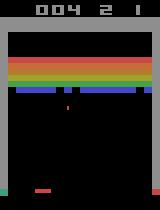
\includegraphics[width=\textwidth]{images/gym-breakout-image-example.jpg}
                \end{figure}
        \end{columns}
    \end{frame}

    \begin{frame}{Q-Learning}
        Q-Learning brief description.
        \begin{equation*}
            Q(S_t, A_t) \leftarrow Q(S_t, A_t) + \alpha \Big[ R_{t+1} +
                \gamma \max_{a} Q(S_{t+1}, a) - Q(S_t, A_t) \Big]
        \end{equation*}
    \end{frame}

    \begin{frame}{SARSA}
        SARSA brief description.
        \begin{equation*}
            Q(S_t, A_t) \leftarrow Q(S_t, A_t) + \alpha \Big[ R_{t+1} +
                \gamma Q(S_{t+1}, A_{t+1}) - Q(S_t, A_t) \Big]
        \end{equation*}
    \end{frame}

    \begin{frame}{$\text{LTL}_f\text{/LDL}_f$ Non-Markovian Rewards}
        $\text{LTL}_f\text{/LDL}_f$ non-Markovian rewards + integration
        in our project.
    \end{frame}

    \section{Implementation}

    \begin{frame}{Robot Features Extraction}
        Algorithms.
    \end{frame}

    \begin{frame}{Goal Features Extraction}
        Algorithms.
    \end{frame}

    \begin{frame}{Temporal Goals}
        Algorithms.
    \end{frame}

    \section{Experiments}

    \begin{frame}{Experiments}
        All the experiments.
    \end{frame}

    \begin{frame}{Conclusion}
        Conclusion.
    \end{frame}

    \begin{frame}[standout]
        Q\&A
    \end{frame}

    \appendix

    \begin{frame}[allowframebreaks]{References}
        \bibliography{bibliography}
        \bibliographystyle{ieeetr}
    \end{frame}

\end{document}
